\subsection{Home Assistant Supervised}\label{sw_hassio}
Nachdem Das Installationsskript (vgl. Abschnitt \ref{ah_skript}: \nameref{ah_skript}) fehlerfrei Home Assistant Supervised installiert hat, können wir mit der Einrichtung fortfahren. 
Dafür öffnen wir, im selben Netzwerk wie unser Raspberry Pi, die Webseite http://<raspberry-pi-adresse>:8123 mit einem beliebigen Browser.\\
\noindent Hier sehen wir einen Anmeldebildschirm (vlg. Abb. \ref{fig:ha1}: \nameref{fig:ha1}) in welchen wir unseren Benutzeraccount mit Passwort für Home Assistant anlegen (vgl. Abb. \ref{fig:ha2}: \nameref{fig:ha2}). 
Anschließend legen wir den Namen und den Standort des Home Assistant fest (vgl. Abb. \ref{fig:ha3}: \nameref{fig:ha3}). 
Der Standort dient der die Ermittlung von Wetterdaten und wird für das Geofencing benötigt. 
Auf dem Nächsten Bildschirm (vgl. Abb. \ref{fig:ha4}: \nameref{fig:ha4}) können wir bereits Vorhandene Smart-Home-Systeme wie Google Cast und Phillips Hue integrieren. 
Da wir allerdings eine eigene Inegration von Zigbee Leuchtmitteln anstreben, wird dieser Schritt übersprungen. 
Nun leitet uns der Home Assistant auf seine Startseite weiter (vgl. Abb. \ref{fig:ha5}: \nameref{fig:ha5}). 
Dieses Dashboard wird von Home Assistant aus allen bereits vorhandenen Geräten bzw. Entitäten generiert. 
\begin{figure}[H]
    \begin{subfigure}{.5\linewidth}
        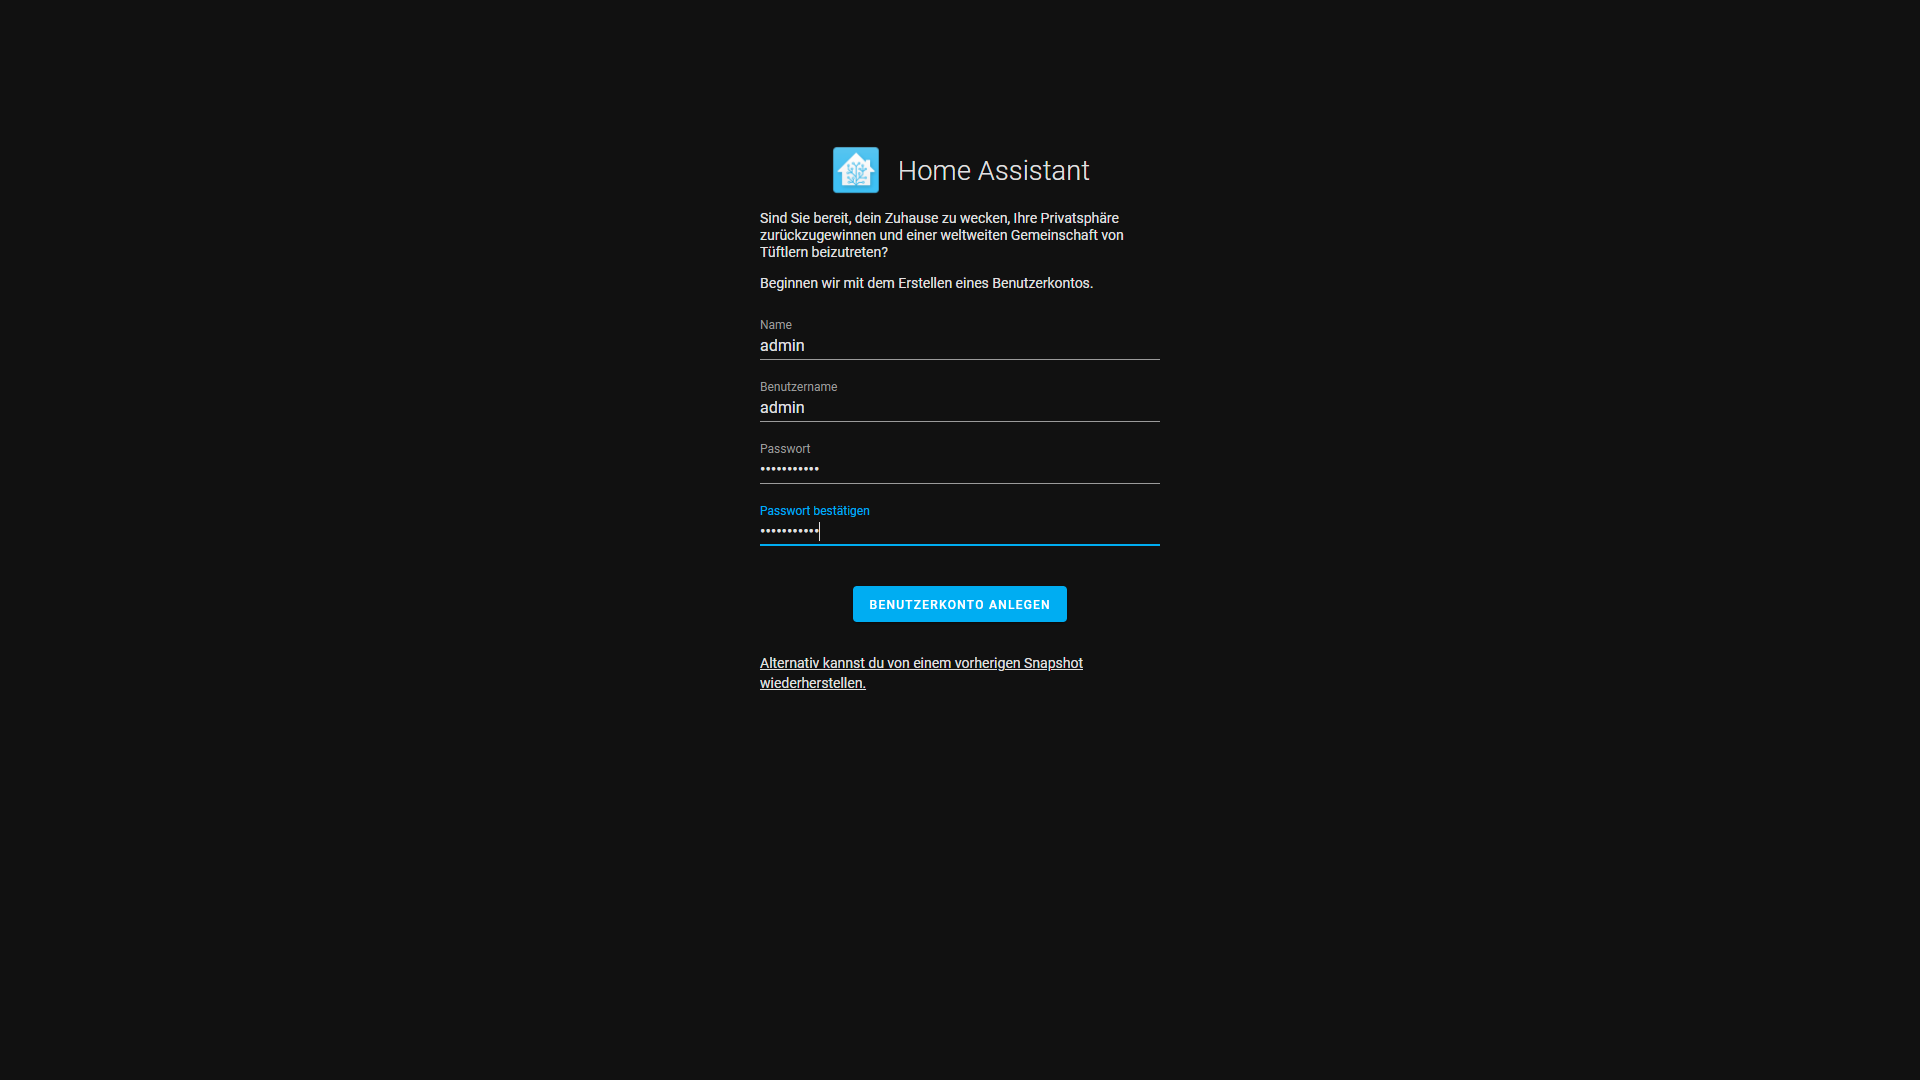
\includegraphics[width=1\textwidth]{img/HA2.png}
        \caption[Anmeldebildschirm]{Anmeldebildschirm}
        \label{fig:ha1}
    \end{subfigure}
    \begin{subfigure}{.5\linewidth}
        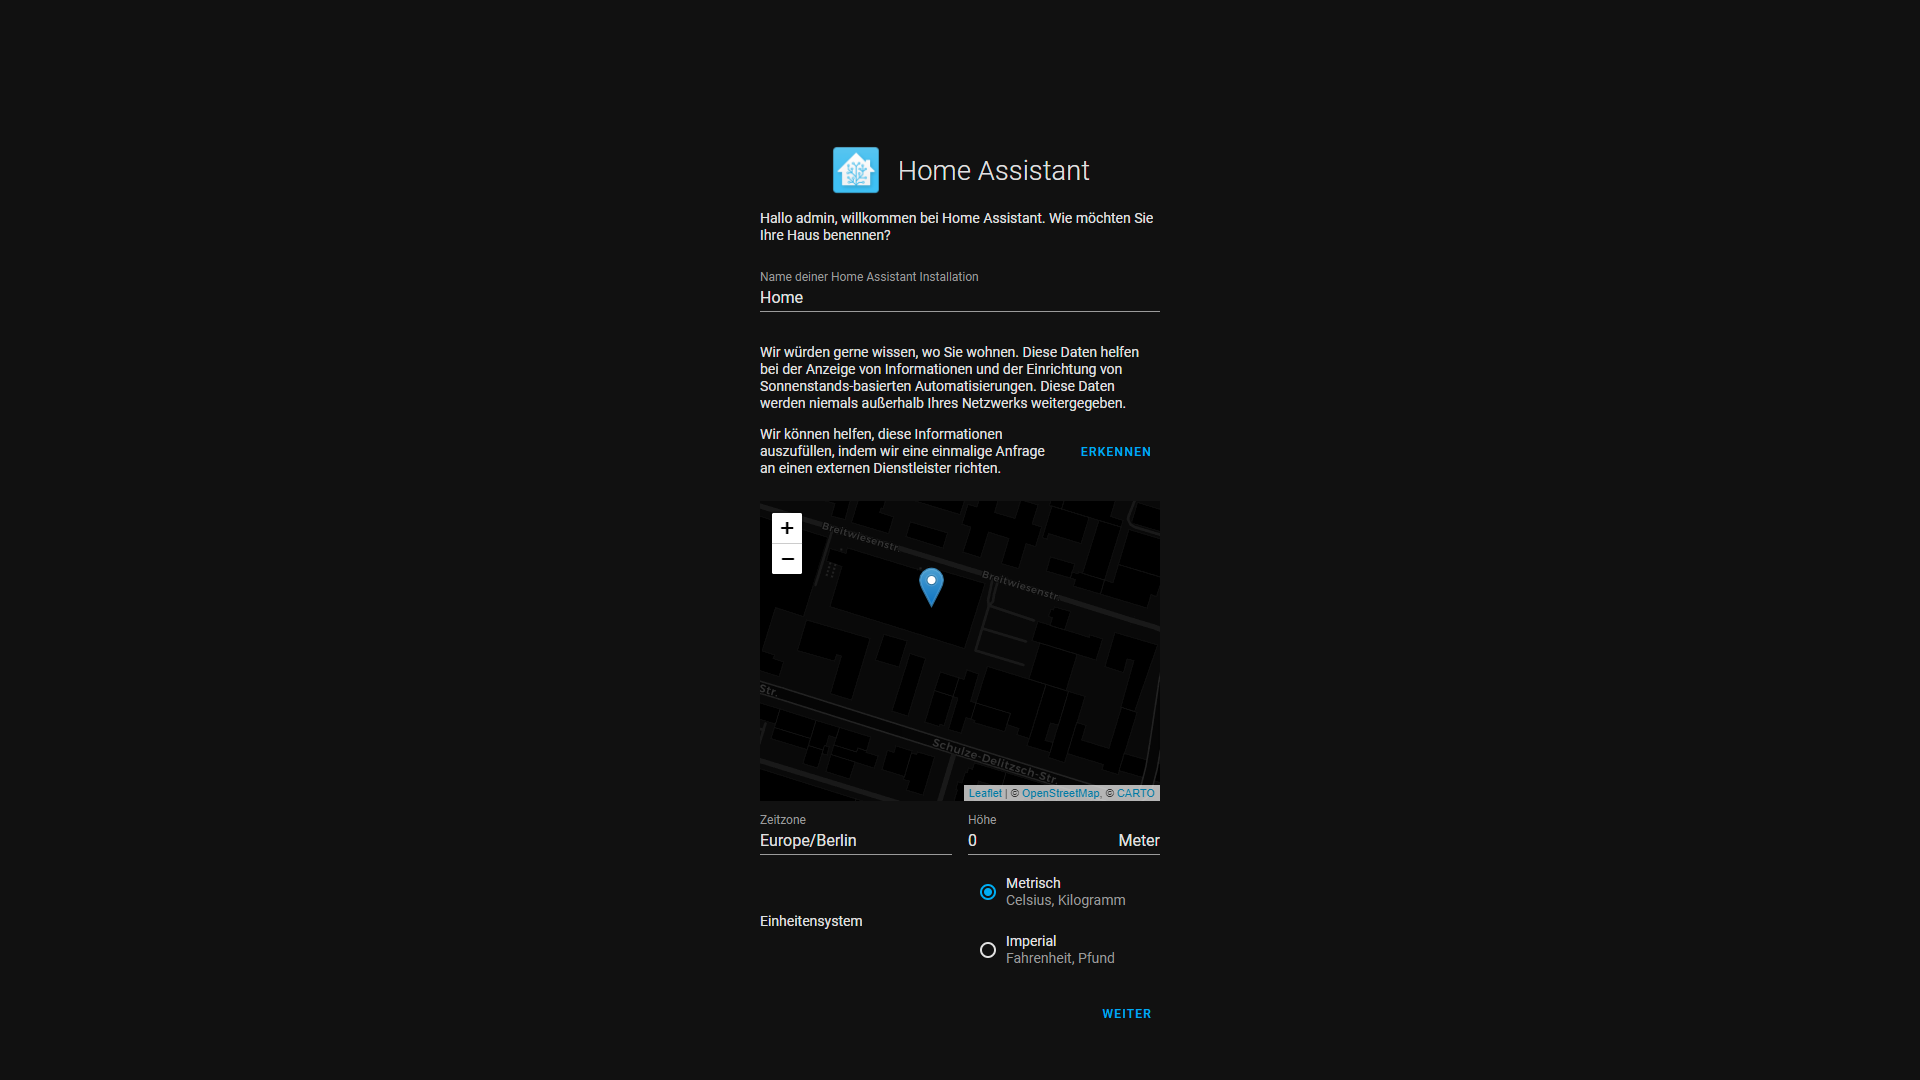
\includegraphics[width=1\textwidth]{img/HA3.png}
        \caption[Festlegen von Name und Standort]{Festlegen von Name und Standort}
        \label{fig:ha2}
    \end{subfigure}
    \begin{subfigure}{.5\linewidth}
        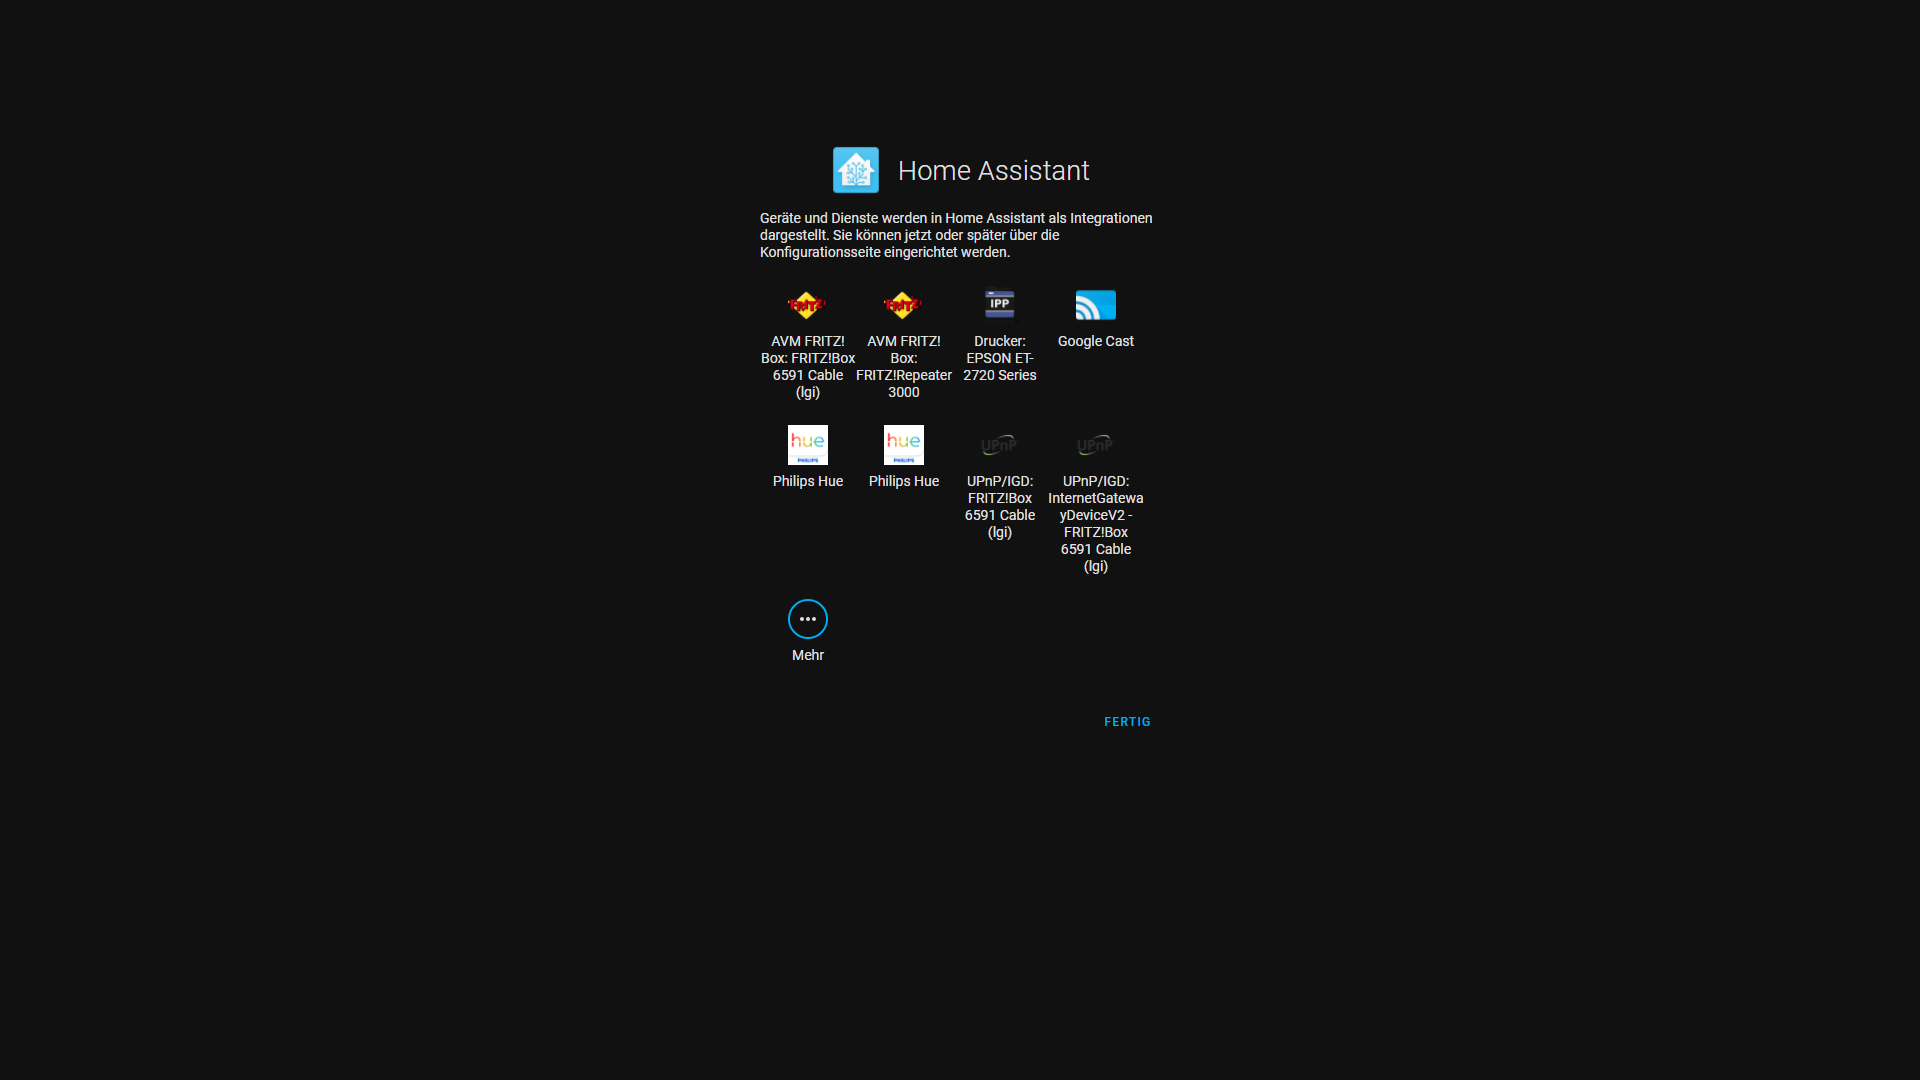
\includegraphics[width=1\textwidth]{img/HA4.png}
        \caption[Mögliche Integrationen werden erkannt]{Mögliche Integrationen werden erkannt}
        \label{fig:ha3}
    \end{subfigure}
    \begin{subfigure}{.5\linewidth}
        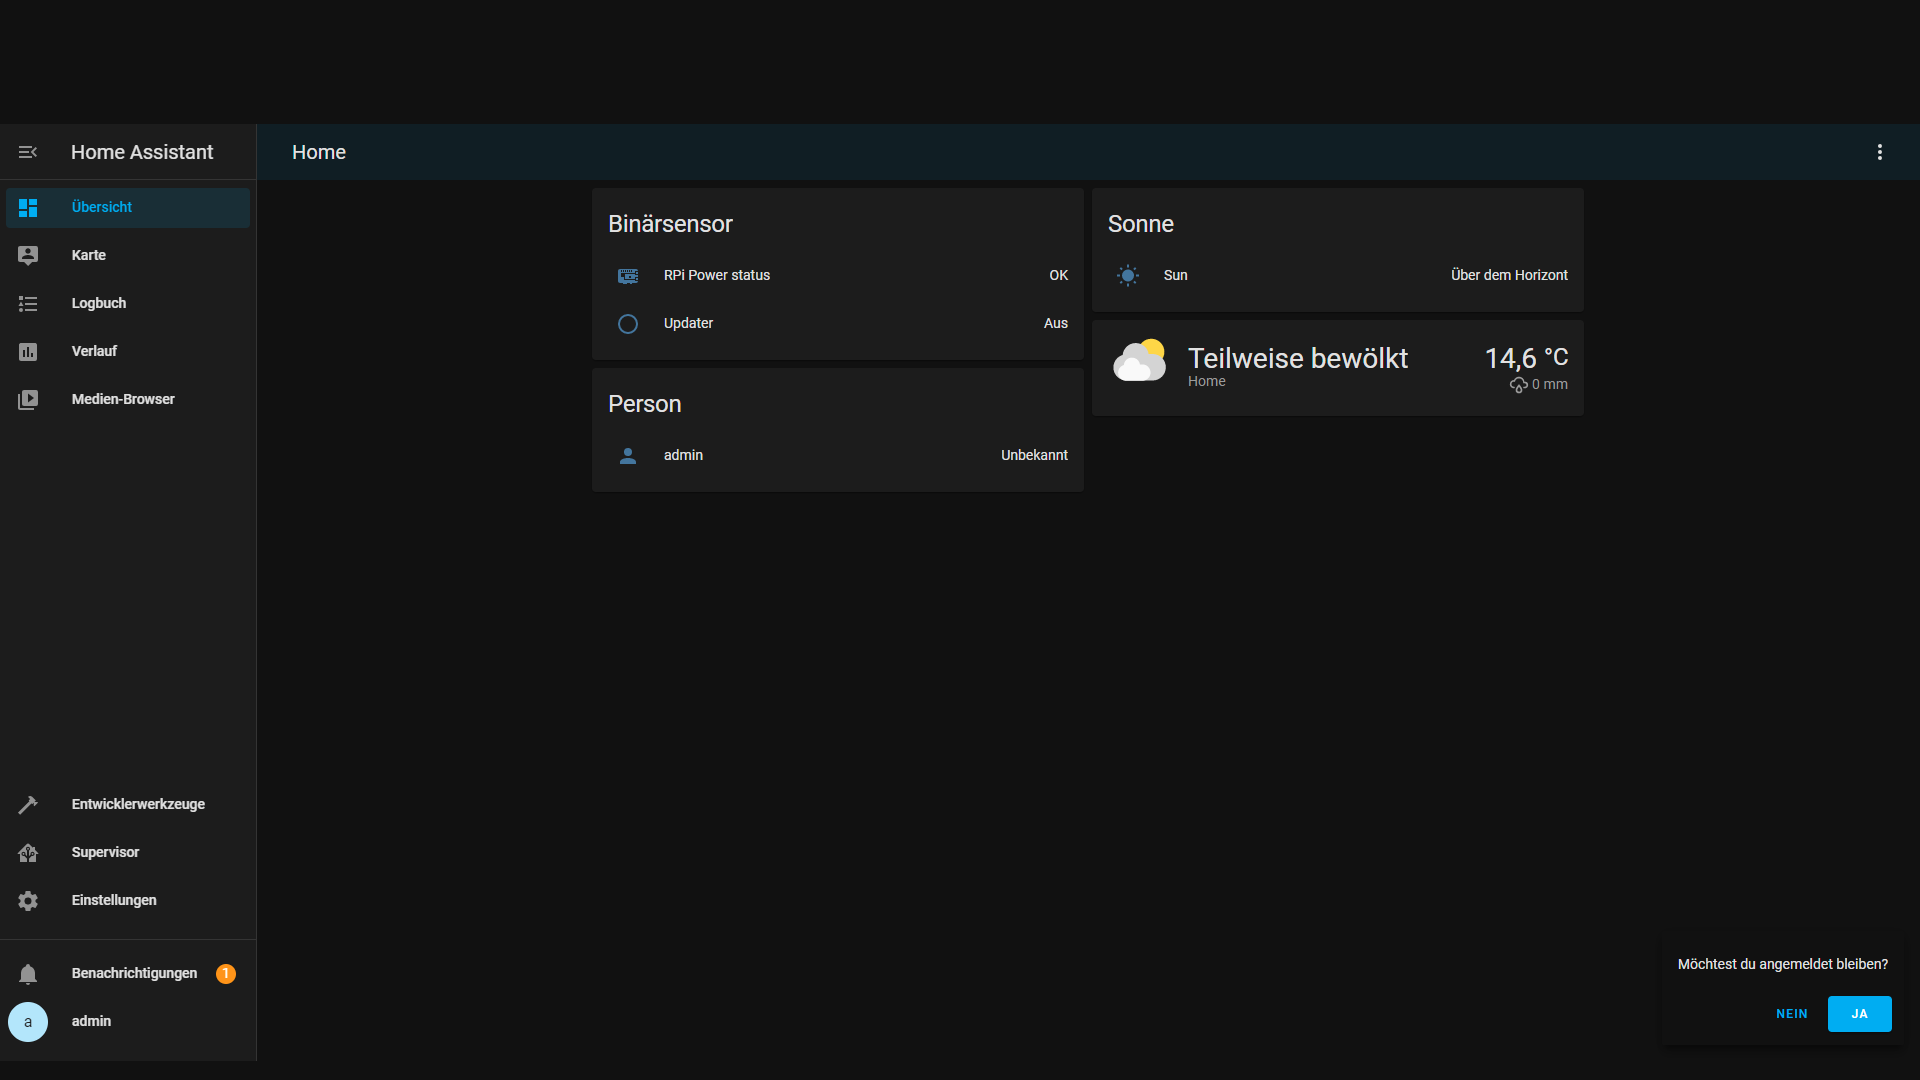
\includegraphics[width=1\textwidth]{img/HA5.png}
        \caption{erstes Dashboard}
        \label{fig:ha4}
    \end{subfigure}
    \label{fig:Einrichtung des Home Assistant}
\end{figure}





